\pagenumbering{arabic}
\section{单表置换密码的加解密}

\subsection{单表置换密码的加解密流程}
\begin{figure}[thbp!]
	\centering
	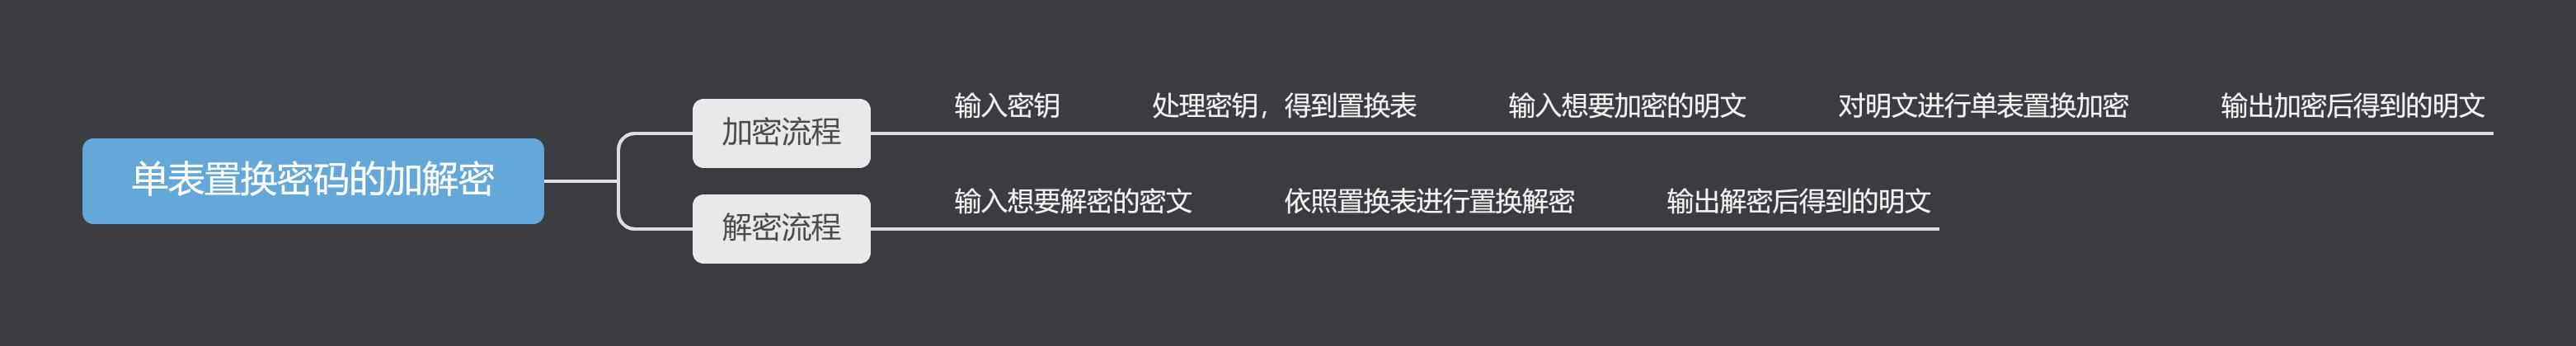
\includegraphics[width=16cm]{figure/figure2.png}
	\caption{单表置换密码的加解密流程}
	\label{fig:单表置换密码的加解密流程}
\end{figure}

\subsection{单表置换密码程序代码}
\begin{lstlisting}[language=c++]
#include <iostream>
#include<string.h>
using namespace std;

//处理输入的密钥
int* build_table(char* inputtext)
{
	int len = strlen(inputtext);
	//输入的密钥长度大于26,则只取前26个
	if (len > 26)
	{
		inputtext[26] = '\0';
		len = 26;
	}
	int* temp = new int[26];
	int j = 0;
	temp[j] = -1;
	for (int i = 0; i < len; i++)
	{
		if (inputtext[i] >= 'A' && inputtext[i] <= 'Z')
		{
			inputtext[i] = inputtext[i] - 'A' + 'a';
		}
		if (inputtext[i] >= 'a' && inputtext[i] <= 'z')
		{
			bool t = true;
			int n = inputtext[i] - 'a';
			for (int k = 0; k <= j; k++)
			{
				if (temp[k] == n)
				{
					t = false;
					break;
				}
			}
			if (t)
			{
				temp[j] = n;
				j++;
			}
		}
	}
	for (int i = 0; i < 26; i++)
	{
		bool t = true;
		for (int k = 0; k < j; k++)
		{
			if (temp[k] == i)
			{
				t = false;
				break;
			}
		}
		if (!t)
			continue;
		else
		{
			temp[j] = i;
			j++;
		}
	}
	//for (int i = 0; i < 26; i++)
	//{
	//    cout << temp[i] << " ";
	//}
	return temp;
}

//解密时使用
int retnum(int* replacetable, int num)
{
	for (int i = 0; i < 26; i++)
	{
		if (replacetable[i] == num)
		{
			return i;
		}
	}
}

class table_replace_crypt
{
private:
	int* replacetable = new int[26];//置换表
public:
	table_replace_crypt()
	{
		for (int i = 0; i < 26; i++)
		{
			replacetable[i] = i;
		}
	}
	table_replace_crypt(char* input)
	{
		replacetable = build_table(input);
	}
	int* getreplacetable()
	{
		return replacetable;
	}
	char* table_replace_encrypt(char*plaintext)//加密
	{
		int len = strlen(plaintext);
		char* ciphertext = new char[len];
		for (int i = 0; i < len; i++)
		{
			if (plaintext[i] >= 'a' && plaintext[i] <= 'z')
			{
				int n = plaintext[i] - 'a';
				ciphertext[i] = plaintext[i] + replacetable[n] - n;
			}
			else if (plaintext[i] >= 'A' && plaintext[i] <= 'Z')
			{
				int n = plaintext[i] - 'A';
				ciphertext[i] = plaintext[i] + replacetable[n] - n;
			}
			else
			ciphertext[i] = plaintext[i];
		}
		ciphertext[len] = '\0';
		return ciphertext;
	}
	char* table_replace_decrypt(char* ciphertext)//解密
	{
		int len = strlen(ciphertext);
		char* plaintext = new char[len];
		for (int i = 0; i < len; i++)
		{
			if (ciphertext[i] >= 'a' && ciphertext[i] <= 'z')
			{
				int n = retnum(replacetable, ciphertext[i] - 'a');
				plaintext[i] = 'a' + n;
			}
			else if (ciphertext[i] >= 'A' && ciphertext[i] <= 'Z')
			{
				int n = retnum(replacetable, ciphertext[i] - 'A');
				plaintext[i] = 'A' + n;
			}
			else
			plaintext[i] = ciphertext[i];
		}
		plaintext[len] = '\0';
		return plaintext;
	}
};
int main()
{
	
	cout << "请输入密钥:";
	char* input = new char[24];
	cin.getline(input, 20);
	
	table_replace_crypt pro = table_replace_crypt(input);
	cout << "置换表为:" << endl;
	for (int i = 0; i < 26; i++)
	{
		cout << char('a' + i) << " ";
	}
	cout << endl;
	int* temp = pro.getreplacetable();
	for (int i = 0; i < 26; i++)
	{
		cout << char('a' + temp[i]) << " ";
	}
	cout << endl << endl;
	
	cout << "请输入要加密的明文:";
	char* plaintext = new char[24];
	char* temp1;
	cin.getline(plaintext, 20);
	temp1 = pro.table_replace_encrypt(plaintext);
	cout << "明文" << plaintext << "加密后的密文为:" << temp1 << endl << endl;
	
	cout << "请输入要解密的密文:";
	char* ciphertext = new char[24];
	char* temp2;
	cin.getline(ciphertext, 20);
	temp2 = pro.table_replace_decrypt(ciphertext);
	cout << "密文" << ciphertext << "解密后的明文为:" << temp2 << endl << endl;
	return 0;
}
\end{lstlisting}


\subsection{程序运行结果}
\begin{figure}[thbp!]
	\centering
	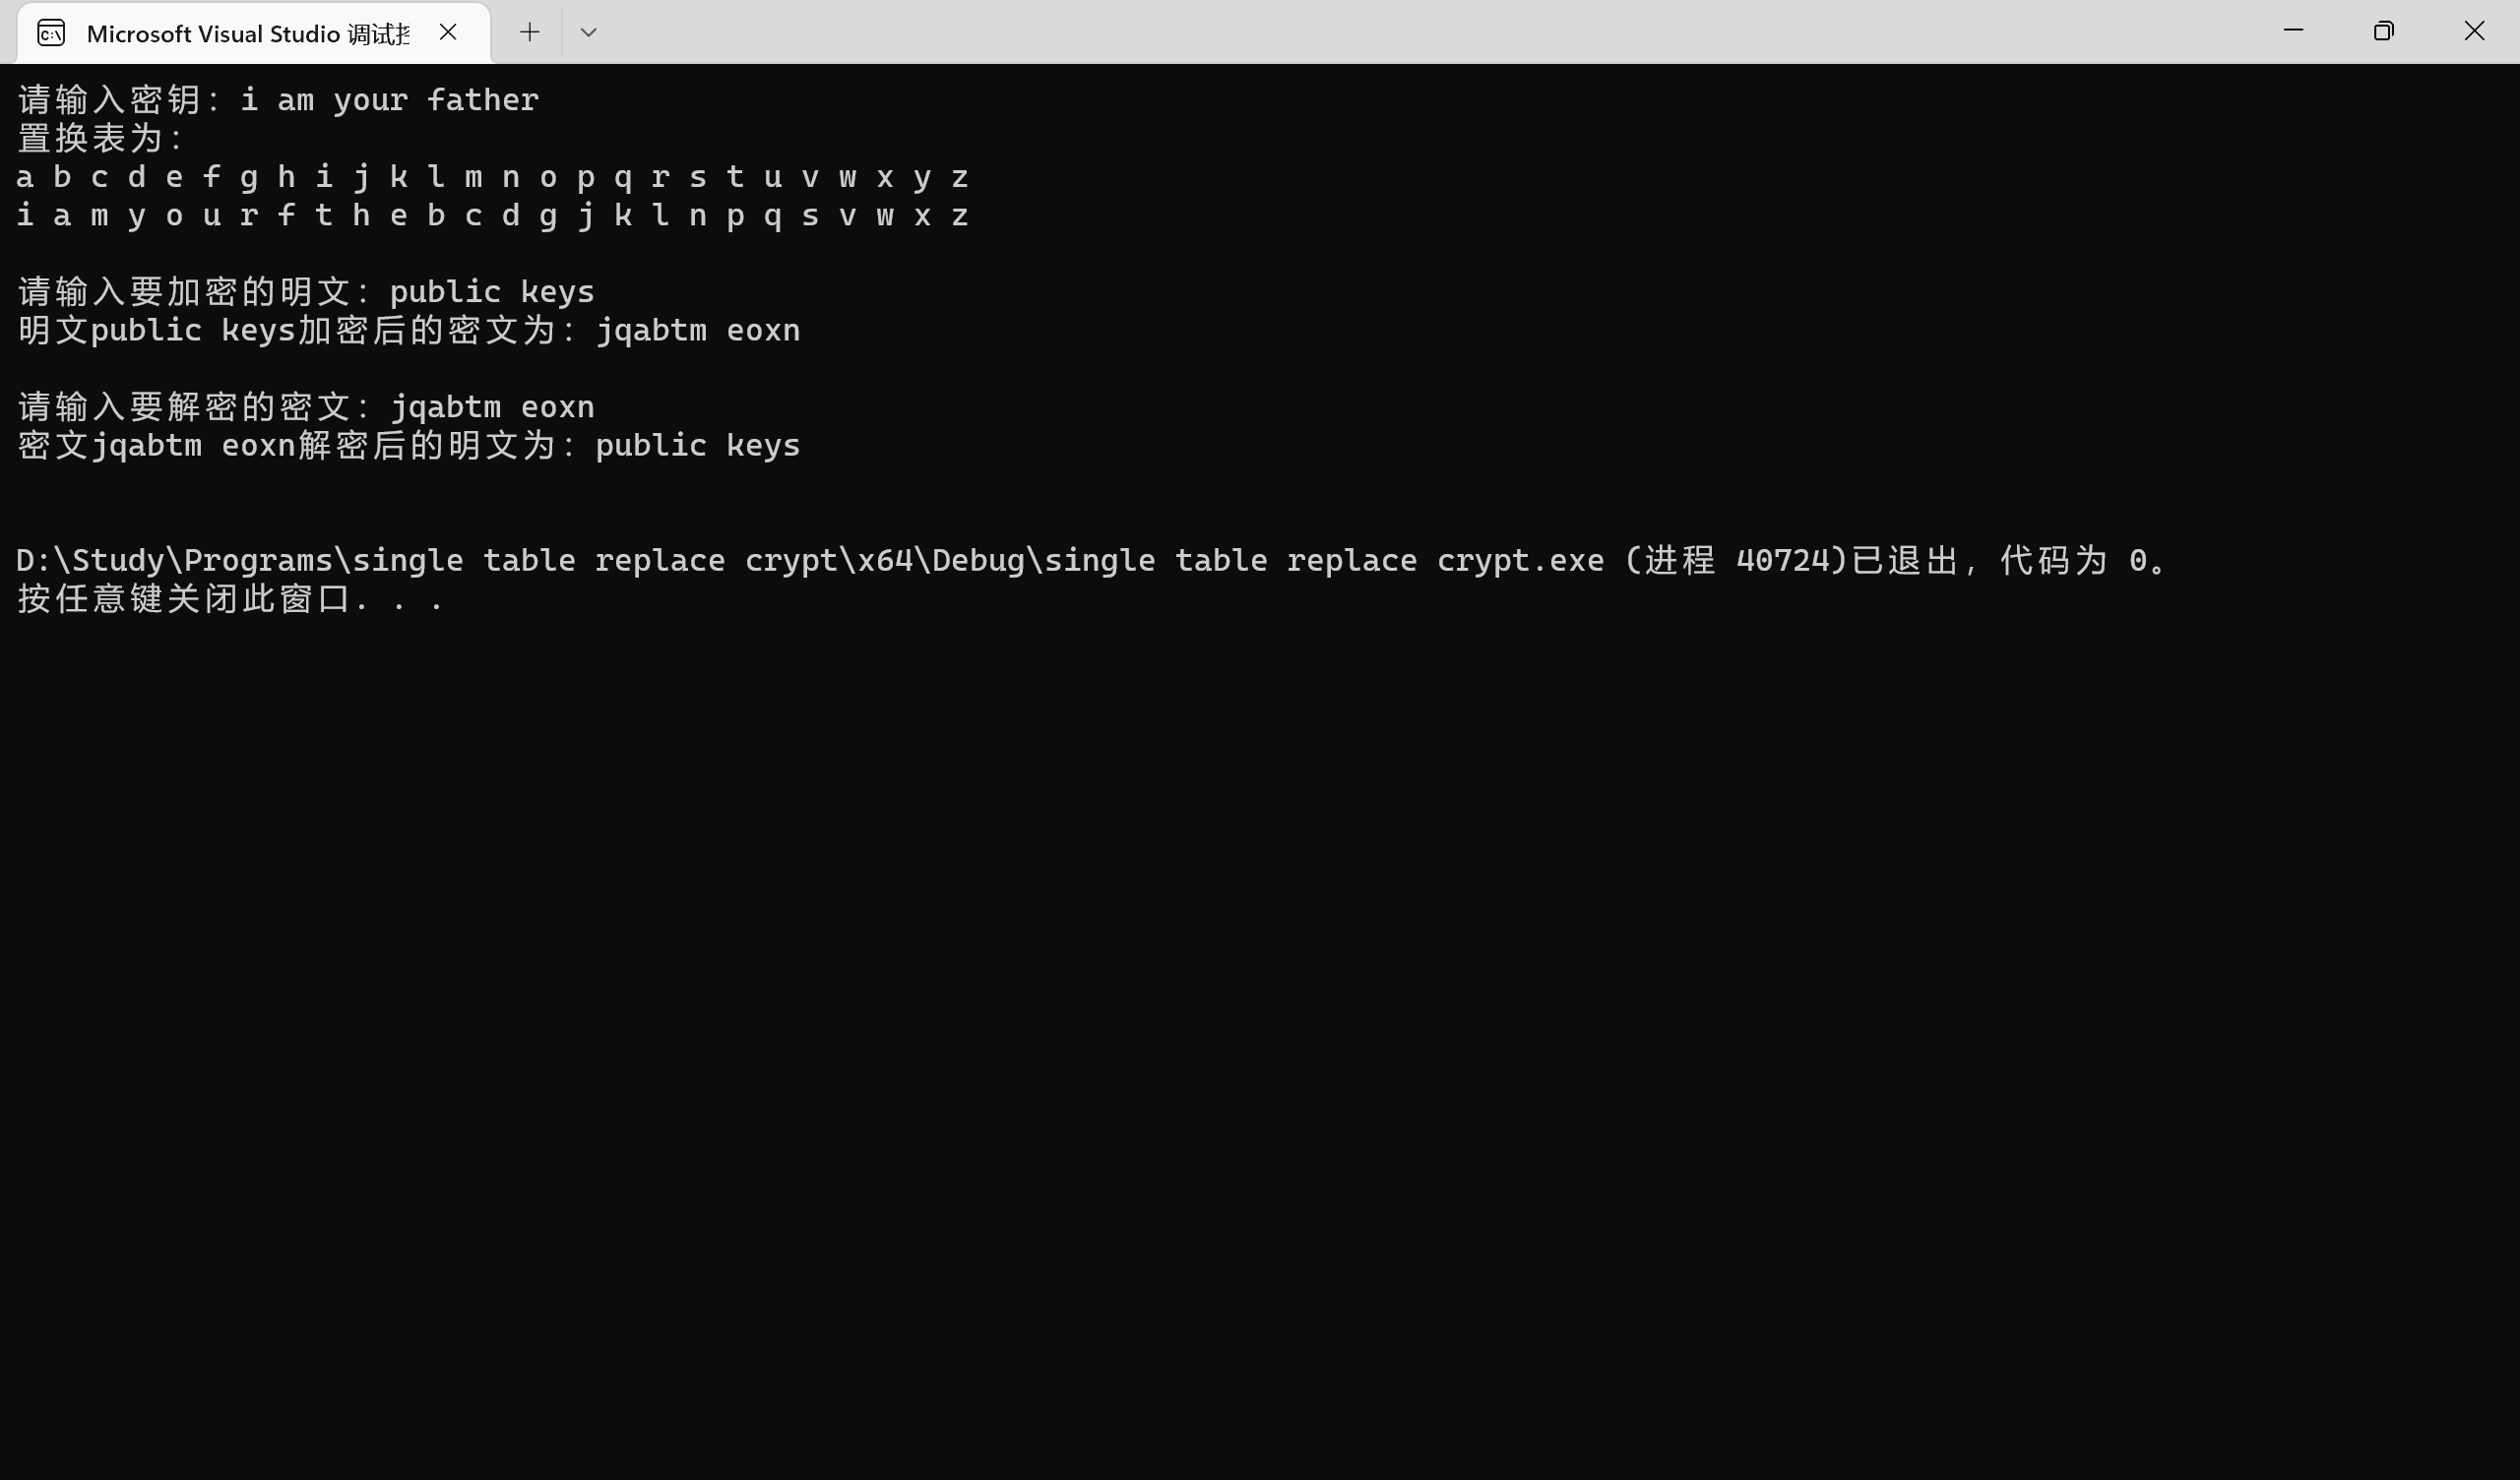
\includegraphics[width=16cm]{figure/003.png}
	\caption{单表置换密码加解密程序运行结果}
	\label{fig:单表置换密码加解密程序运行结果}
\end{figure}

%\begin{enumerate}
%	\item \textbf {预处理器:}处理源代码中以\#开始的预编译指令,例如展开所有宏定义、插入\#include指向的文件等,以获得经过预处理的源程序。
%	
%	\item \textbf {编译器:}将预处理器处理过的源程序文件翻译成为标准的汇编语言以供计算机阅读。
%	
%	\item \textbf {汇编器:}将汇编语言指令翻译成机器语言指令,并将汇编语言程序打包成可重定位目标程序。
%	
%	\item \textbf {链接器:}将可重定位的机器代码和相应的一些目标文件以及库文件连接在一起,形成真正能在机器上运行的目标机器代码。
%\end{enumerate}

%\begin{figure}[thbp!]
%	\centering
%	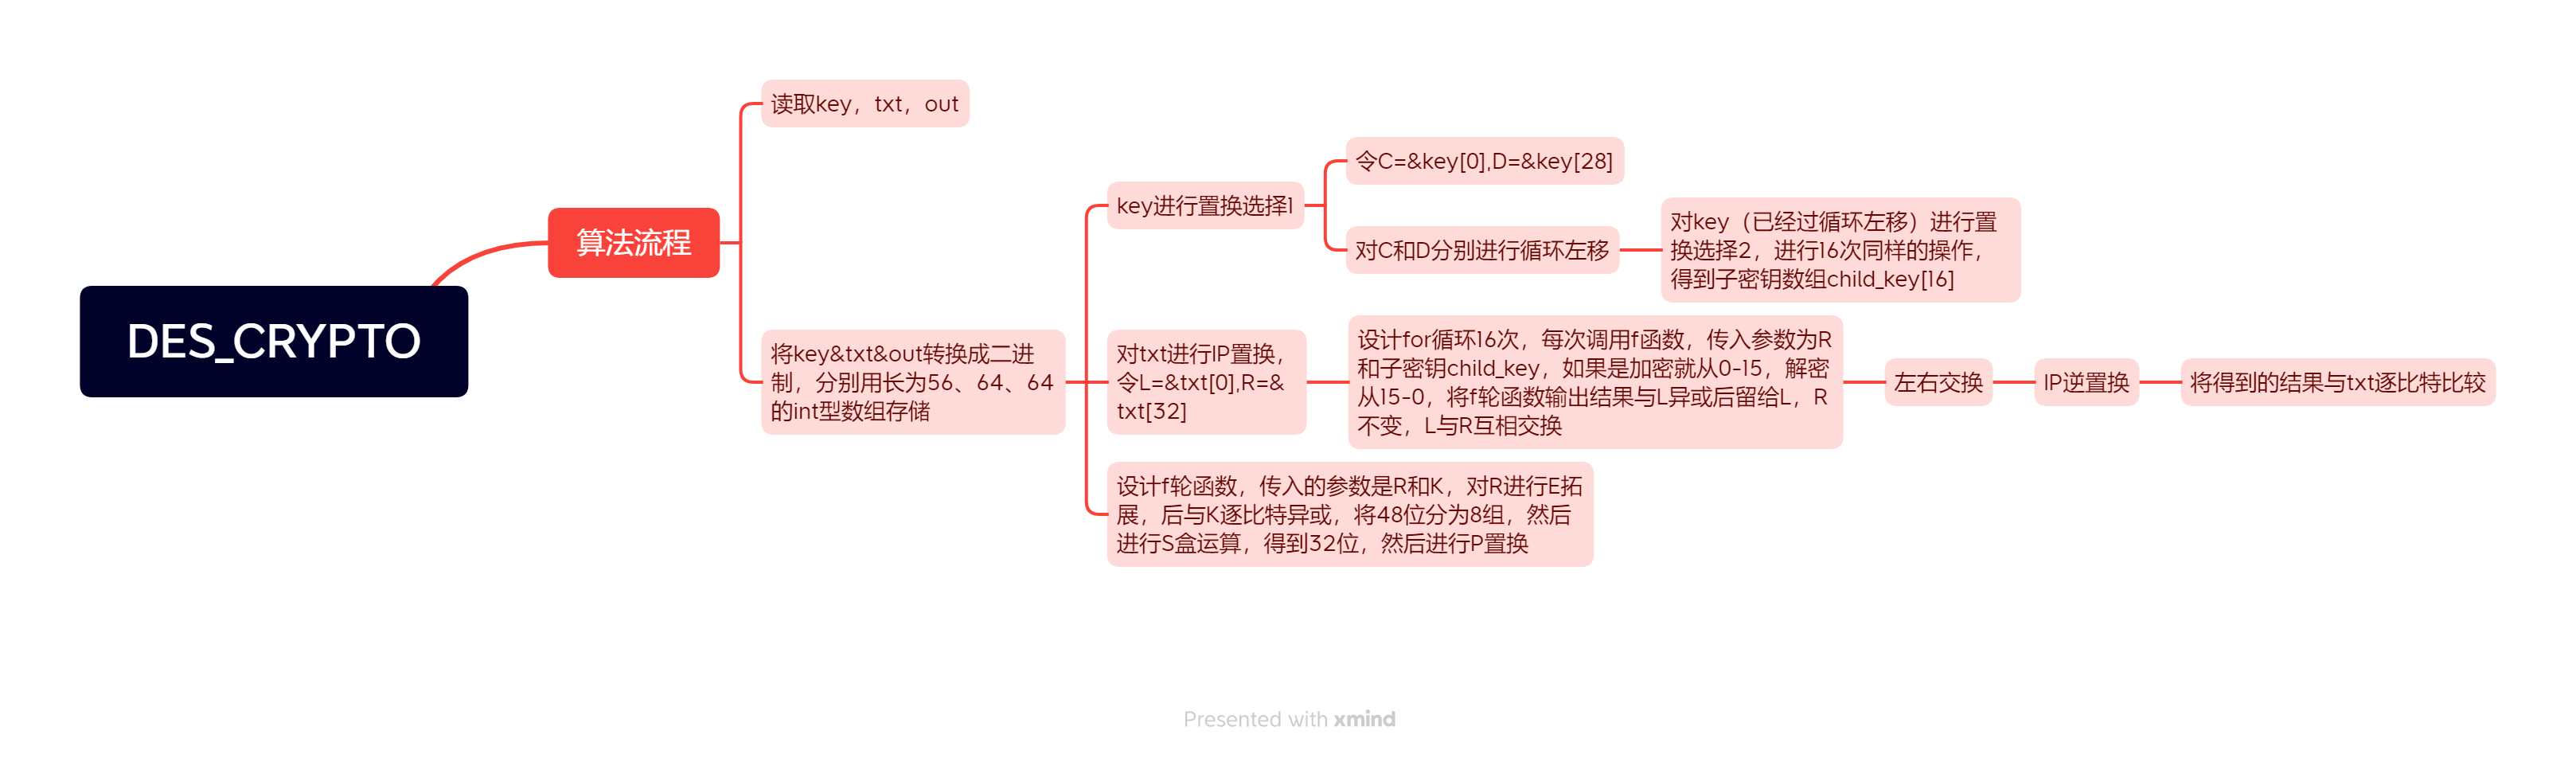
\includegraphics[height=6.8 CM]{figure/001}
%	\caption{语言处理过程图示}
%	\label{fig:语言处理过程图示}
%\end{figure}

























